\documentclass{article}
\usepackage[utf8]{inputenc}
\usepackage{pmboxdraw}
\usepackage[english, danish]{babel}
\usepackage{graphicx}
\usepackage{graphics}
\usepackage{caption}
\usepackage{subcaption}
\usepackage{hyperref}
\usepackage[]{algorithm2e}
\usepackage{listings}
\usepackage{lineno}
\usepackage{amssymb}
\usepackage{amsmath}
\usepackage{listings}
\usepackage{upquote}
\usepackage{color}
\definecolor{bluekeywords}{rgb}{0.13,0.13,1}
\definecolor{greencomments}{rgb}{0,0.5,0}
\definecolor{redstrings}{rgb}{0.9,0,0}
 
\lstdefinelanguage{FSharp}%
{morekeywords={let, new, match, with, rec, open, module, namespace, type, of, member, % 
and, for, while, true, false, in, do, begin, end, fun, function, return, yield, try, %
mutable, if, then, else, cloud, async, static, use, abstract, interface, inherit, finally },
  otherkeywords={ let!, return!, do!, yield!, use!, var, from, select, where, order, by },
  keywordstyle=\color{bluekeywords},
  sensitive=true,
  basicstyle=\ttfamily,
	breaklines=true,
  aboveskip=\bigskipamount,
	tabsize=2,
  morecomment=[l][\color{greencomments}]{////},
  morecomment=[l][\color{greencomments}]{///},
  morecomment=[s][\color{greencomments}]{{(*}{*)}},
  morestring=[b]",
  showstringspaces=false,
  literate={`}{\`}1,
  stringstyle=\color{redstrings},
  texcl=true
}


\title{7g rapport}
\author{Emil Henriksen wsl798,\\ Jonathan Gabel Christiansen dvg554\\ og Jens Evald-Schelde  xfb949}
\date{November 2018}

\begin{document}

\maketitle
\newpage
\section*{Introduction}
We have been given the task to implement the game Awari in F\#.
Awari is an African boardgame that is played by 2 players with 7 sticks and 36 beans. The sticks are placed so that they create 14 pits, where 2 are homepits. The beans are distributed in all but the homepits, so that each pit contains 3 beans.\\
A turn is played by picking up all the beans from one of the players pits and distributing them counterclockwise by placing one in each of the following pits including the home pits.\\
If the last bean is placed in the players homepit the player gets another turn.\\
If the last bean is placed in an empty pit that is not the the hompit, all the beans from the pit on the opposite site is catched and placed in the players homepit.\\
The game is over when one of the players pits are empty.

\begin{figure}[h]
  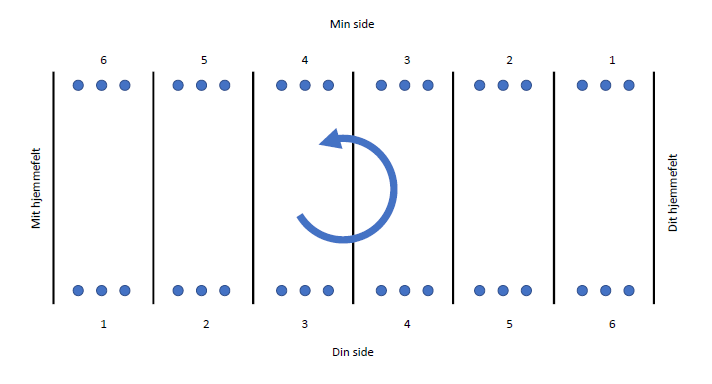
\includegraphics[width=\linewidth]{awari.jpg}
  \caption{awari.jpg}
  \label{fig:A picture of Awari}
\end{figure}

\section{Design and implementation}
In this section we describe our game implementation.\\
\subsection*{Types}
The game is built around the 3 types:
\lstset{language=Python,numbers=left,stepnumber=1}
\begin{lstlisting}[frame=single]
type pit = {mutable cell: int; id:int}
type board = {pits:pit list}
type player = Player1 | Player2
\end{lstlisting}
"Pit" is simply a type containing a mutable cell with an ID which increments from 0 up to 13. Each cell contains an integer. It's mutable because our game revolves around the fact that the cells can be changed.\\
"Board" is a list of pits. The board contains pits that can be changed. So that when beans are distributed, catched etc. the pits within the board can be updated with the correct values.\\
"Player" is an enumeration. It contains 2 values which we define as Player1 and Player2. This is done since the names are meaningful in the game context and integers such as 0 and 1 are not.
\subsection*{Library}
In this section we describe the functions in our library. We do so to make it clear what the functions do when describing the application in the next section.\\
\\
printBoard : b:board $\rightarrow$ unit\\
The function printBoard simply prints a board to the console. Since we have defined a board as an list, the function simply prints elements 0-5 as player 1's pits, elements 7-12 as player 2's pits and lastly elements 6 and 13 as homepits.
It does so using the built in list functions List.iter, List.rev and list indexing. \textbackslash n makes sure that player1's pits, player2's pits and homepits are printed on individual lines, so that the game looks like the real one.\\
\\
isHome : b:board$\rightarrow$ p:player $\rightarrow$ i:pit $\rightarrow$ bool\\
The function isHome checks if a pit is the homepit of a player. It does so by checking if the pit is element 6 in the list AND if the player is Player1 or the same procedure with element 13 AND Player2. If both conditionals are true in each case it returns true.
Else false.\\
\\
isGameOver : b:board $\rightarrow$ bool\\
The function checks if elements 0-5 all are equal to 0 for Player1 OR if the elements 7-12 all are equal to 0 for Player2. It does so using the built-in list function List.forall.\\ If either of the cases are true the game is over. If none of the cases are true the game is still going.\\
\\
distribute : b:board $\rightarrow$ p:player $\rightarrow$ i:pit $\rightarrow$ board * player * pit\\
The distribute function serves to distribute beans counter clockwise from the chosen pit.
It starts by setting the chosen pit to 0 (all the beans are picked up from this pit) and then distributes beans 1 at a time in the following pits corresponding to the amount of beans picked up.\\
Example: if 3 beans are picked up from pit 3 on the board, it will increment pits 4,5,6 on the board by 1 and since the board is an int list, the function increments the pits by using list indexing.\\
The capture is implemented by checking the last pit to have a bean placed in it has value 1 (0+1) AND if the bean placed is on the players side AND that it's the corresponding player. If so the players homepit is incremented by the values from the 2 opposing pits. It finds the opposing pit by calculating 12-pit.id. 
Example: player 1 lands in empty pit 2 and we capture the opposing side (12-2=10) and put all the beans in pit 6.\\

getMove : b:board $\rightarrow$ p:player $\rightarrow$ q:string $\rightarrow$ pit\\
When the player types his/her move into the console, the input is casted to type int. The function checks if its a valid input. Valid input are as follows\\
Player1 : $1 \leq \text{ input } \leq 6$\\
Player2 : $1 \leq \text{ input } \leq 6$\\
In both cases if the input is outside of the interval, the value will be changed to the closest value within the interval.\\
For Player2 the output is input converted to zero indexing +7. This is done to ease the gameplay. In short both players only have to remember that their pits are named 1-6 instead of them having different names.\\
Example:\\
If Player2 types in "7", 7 will be changed to 5 since there are only 6 pits (0-indexing) and then the input will be added to 7. So Player2 has chosen his 6th pit which is corresponding to the 12th element in the list.\\
\\
turn : b:board $\rightarrow$ p:player $\rightarrow$ board\\
The function turn encapsulates a recursive function repeat. It's recursive because it calls itself every turn. Alternating between players or giving extra turns. The function starts by printing an updated board every turn. The function then takes user input (a move from one of the players) and calls getMove to get the corresponding pit. The function then calls distribute with the current board, player and the pit we got from getMove. If the pit that is returned isn't the players homePit OR the game isn't over then the game continues  with an updated board, the next player and an integer determining if it's either Player1 or Player2. If it is the players homePit or the game is over it either provides an extra turn or ends the game.\\
\\
play : b:board $\rightarrow$ p:player $\rightarrow$ board\\
The recursive function play starts by calling the function isGameOver, if true is returned, the final board is printed and the game is over.\\
If it's false a new board is printed and the next players gets his/hers turn by calling the function turn.\\
The function calls itself until the game is over.

\subsection*{Application}
The application is fairly simple. Awari.fsx opens the module Awari and calls printBoard with the function play, a board which is already defined and Player1 (the starting player).
When the function is compiled with Awari.dll and run with mono the game can be played in the console.\\
The game is presented in the console with a board and 2 lines of text "6 5 4 3 2 1" and "1 2 3 4 5 6" corresponding to the number the player has to input to chose the pit below or above.\\
Player 1 is at the bottom and player 2 is at the top. Player 1 has the rightmost homepit and player 2 has the leftmost.
\section*{Testing}
This section contains a walktrough our whitebox testing one function at a time.
We've tested the functions according to the game rules and we aim to test every line of code.\\
\\
printBoard:\\
This function is tested through other functions since it just prints the board.\\
\\
isHome:\\
We've tested if it returns true when landing in either Player1 or Player2s homepit. We've also tested if it returns false if it lands in an ordinary pit.\\
\\
isGameOver:\\
We've tested if it returns true when one of the players pits are empty and if it returns false when there are still beans on both sides.\\
\\
getMove:\\
We've tested correct inputs from both players, too large inputs from both players and lastly too small inputs from both players. We haven't tested non-numerical characters. These inputs results in an exception.\\
\\
distribute:\\
We've tested 1 ordinary move (without capturing) for each player, 1 move from each player with capturing and 1 move from each player where the last bean is placed in their homepit resulting in an extra turn.\\
\\
turn and play takes user input and have not been tested like the rest of our functions.
\\
\lstset{xleftmargin=-50pt,xrightmargin=-50pt}
\pagebreak
\section*{Appendix}
\subsubsection{Awari.fs}
\lstset{language=FSharp,numbers=left,stepnumber=1}
\begin{lstlisting}[frame=single]
module Awari
open System
type pit = {mutable cell:int;id:int}
type board = {pits:pit list}
type player = Player1 | Player2

let b = {pits= [for i in 0..13 -> {cell=3;id=i}]}
// Setting Home pits to zero
b.pits.[6].cell <-  0
b.pits.[13].cell <- 0

/// <summary>The function to draw our game board on screen</summary>
/// <param name="b">b: is a board holdning pits</param>
/// <remarks> At the moment it will only work with a specific size board</remarks>
/// <returns> A printed representation of the current game board</returns>
let printBoard (b:board) =
  /// Getting Graphic for this one!
  Console.BackgroundColor <- ConsoleColor.Black
  Console.ForegroundColor <- ConsoleColor.Red
  printfn """  
 █████╗ ██╗    ██╗ █████╗ ██████╗ ██╗
██╔══██╗██║    ██║██╔══██╗██╔══██╗██║
███████║██║ █╗ ██║███████║██████╔╝██║
██╔══██║██║███╗██║██╔══██║██╔══██╗██║
██║  ██║╚███╔███╔╝██║  ██║██║  ██║██║
╚═╝  ╚═╝ ╚══╝╚══╝ ╚═╝  ╚═╝╚═╝  ╚═╝╚═╝"""
  Console.ResetColor()
  printfn "q to quit\n"
  
  // Starting to print board
  List.iter (fun x -> printf "%s" x) [for i in 1..6 -> "____"]
  printfn ""
  List.rev [for i in 1..6 -> i] |> List.iter (fun x -> printf "%3i|" x)
  printfn "P2"
  List.iter (fun x -> printf "%s" x) [for i in 1..6 -> "‾‾‾‾"]
  printfn ""
  // Printing player 1 board side
  Console.ForegroundColor <- ConsoleColor.Black
  Console.BackgroundColor <- ConsoleColor.DarkRed
  b.pits.[7..12] |> List.rev |> List.iter (fun x -> printf "%3i|" x.cell)
  printf "   "
  // Reseting the console to default
  Console.ResetColor()
  printfn ""
  // Printing players home pits
  Console.ForegroundColor <- ConsoleColor.Black
  Console.BackgroundColor <- ConsoleColor.DarkYellow
  printf "%-4i%23i" b.pits.[13].cell b.pits.[6].cell
  // Reseting the console to default
  Console.ResetColor()
  printfn ""
  // Printing player 2 board side
  Console.ForegroundColor <- ConsoleColor.Black
  Console.BackgroundColor <- ConsoleColor.DarkRed
  b.pits.[..5] |> List.iter (fun x -> printf "%3i|"  x.cell)
  printf "   "
  // Reseting the console to default
  Console.ResetColor()
  printfn ""
  List.iter (fun x -> printf "%s" x) [for i in 1..6 -> "____"]
  printfn ""
  List.iter (fun x -> printf "%3i|" x) [for i in 1..6 -> i]
  printfn "P1"
  List.iter (fun x -> printf "%s" x) [for i in 1..6 -> "‾‾‾‾"]
  printfn ""

/// <summary>The function will check if a pit belongs to a player</summary>
/// <param name="b">b: is a board holdning pits</param>
/// <param name="p">p: is a player</param>
/// <param name="i">i: is a pit</param>
/// <remarks> At the moment it will only work with a specific size board</remarks>
/// <returns> A bool</returns>   
let isHome (b:board) (p:player) (i:pit) : bool =
  if (i.id = b.pits.[6].id && p = Player1) then 
    true
  elif (i.id = b.pits.[13].id && p = Player2) then
    true
  else false

/// <summary>The function will check the baord to see if it's game over</summary>
/// <param name="b">b: is a board holdning pits</param>
/// <remarks> At the moment it will only work with a specific size board</remarks>
/// <returns> A bool</returns> 
let isGameOver (b:board) : bool =
  b.pits.[..5] |> List.forall (fun x -> x.cell = 0) || 
  b.pits.[7..12] |> List.forall (fun x -> x.cell = 0)

/// <summary>This function will distribute all them beans</summary>
/// <param name="b">b: is a board holdning pits</param>
/// <param name="p">p: is a player </param>
/// <param name="i">i: is pit </param>
/// <remarks> Has not been tested with anything but standard board size, 
/// but should work for almost any size</remarks>
/// <returns>A tuple of a changed board, the player and the pit</returns>
let distribute (b: board) (p:player) (i:pit) : board * player * pit =
  let mutable hand = i.cell
  i.cell <- 0
  // moveCount keeps track of placement, starting with the pit next to the chosen one!
  let mutable moveCount = i.id+1
  // 'move' makes sure to wrap around, so the list is more like an circle, 
  // and we need it both in the while loop and outside. The scope is important.
  let mutable move = moveCount%(b.pits.Length)

  while not(hand = 0) do
    move <- moveCount%(b.pits.Length)
    moveCount <- moveCount + 1
    if (isHome b p b.pits.[move]) then
      b.pits.[move].cell <- b.pits.[move].cell + 1
      hand <- hand-1

    elif (p=Player1) && not (isHome b Player2 b.pits.[move]) then
      b.pits.[move].cell <- b.pits.[move].cell + 1
      hand <- hand-1

    elif ( p=Player2) && not (isHome b Player1 b.pits.[move]) then
      b.pits.[move].cell <- b.pits.[move].cell + 1
      hand <- hand-1
  
  // Catching the opposing sides beans if the last bean is placed in 
  // an empty pit on the players home field. The opposing side will always be 12 minus the pit
  if(b.pits.[move].cell = 1 && b.pits.[move].id <= 5 && p = Player1) then
    b.pits.[6].cell  <- b.pits.[12-move].cell + b.pits.[6].cell + b.pits.[move].cell
    b.pits.[12-move].cell <- 0
    b.pits.[move].cell <- 0

  elif(b.pits.[move].cell = 1 && b.pits.[move].id >= 7 && p = Player2 && not(isHome b Player2 b.pits.[move])) then
    b.pits.[13].cell <- b.pits.[12-move].cell + b.pits.[13].cell + b.pits.[move].cell
    b.pits.[12-move].cell <- 0
    b.pits.[move].cell <- 0

  // Winner Winner Chicken Dinner! You get it all!
  if (isGameOver b) then 
    if (p=Player1) then
      let win = b.pits.[7..12] |> List.fold (fun acc x -> x.cell + acc) 0
      b.pits.[6].cell <- b.pits.[6].cell + win
      for i in 7..12 do
        b.pits.[i].cell <- 0
    else 
      let win = b.pits.[..5] |> List.fold (fun acc x -> x.cell + acc) 0
      b.pits.[13].cell <- b.pits.[13].cell + win
      for i in 1..5 do
        b.pits.[i].cell <- 0
  (b,p,b.pits.[move])


/// <summary>This function will get the players move</summary>
/// <param name="b">b: is a board holdning pits</param>
/// <param name="p">p: is a player </param>
/// <param name="q">q: is a string with the move </param>
/// <remarks> Has not been tested with anything but standard board size, 
/// but should work for almost any size</remarks>
/// <returns> A pit</returns>
let getMove (b:board) (p:player) (q:string) : pit =
  let mutable qInt = 0
  if (q = "q" || q = "Q") then Environment.Exit 1
  else qInt <- int32(q)-1
  // 6 could have been represented as a variable since it always (b.pits.Length/2) 
  // and 5 could have been (b.pits.Length/2)-1
  if (qInt >= 6) then qInt <- 5
  elif (qInt <= 0) then qInt <- 0
  // +7 could also have been a variable containg the value of "(b.pits.Length/2)+1" 
  // This way the game would scale well. 
  if p = Player1 then b.pits.[qInt]
  else b.pits.[qInt+7]


/// <summary>This function will get the players move</summary>
/// <param name="b">is a board holdning pits</param>
/// <param name="p">is a player </param>
/// <param name="q">is a string with the move </param>
/// <remarks> Has not been tested with anything but standard board size, 
/// but should work for almost any size</remarks>
/// <returns> A pit</returns>
let turn (b : board) (p : player) : board =
  let rec repeat (b: board) (p: player) (n: int) : board =
    printBoard b
    let str =
      if n = 0 then
        printf "%A's move? " p
        Console.ReadLine()
      else 
        printf "Extra Move %A " p
        Console.ReadLine()
    let i = getMove b p str
    let (newB, finalPitsPlayer, finalPit)= distribute b p i
    if not (isHome b finalPitsPlayer finalPit) 
       || (isGameOver b) then
      System.Console.Clear()
      newB
    else
      System.Console.Clear()
      repeat newB p (n + 1)
  repeat b p 0 


/// <summary>This function will play</summary>
/// <param name="b">is a board holdning pits</param>
/// <param name="p">is a player </param>
/// <remarks> Has not been tested with anything but standard board size, 
/// but should work for almost any size if scale is wanted</remarks>
/// <returns> A board</returns>
let rec play (b : board) (p : player) : board =
  if isGameOver b then
    b
  else
    let newB = turn b p
    let nextP =
      if p = Player1 then
        Player2
      else
        Player1
play newB nextP
\end{lstlisting}

\subsubsection{Awari.fsi}
\lstset{language=FSharp,numbers=left,stepnumber=1}
\begin{lstlisting}[frame=single]
module Awari

type pit = {mutable cell: int; id: int}

type board =  {pits: pit list;}

type player = Player1 | Player2

val printBoard : b:board -> unit

val isHome : b:board -> p:player -> i:pit -> bool

val isGameOver : b:board -> bool

val getMove : b:board -> p:player -> q:string -> pit

val distribute : b:board -> p:player -> i:pit -> board * player * pit

val turn : b:board -> p:player -> board

val play : b:board -> p:player -> board
\end{lstlisting}
\subsubsection{Awari.fsx}
\lstset{language=FSharp,numbers=left,stepnumber=1}
\begin{lstlisting}[frame=single]
open Awari
// Starting game by getting it to print the last board
printBoard (play b Player1)
\end{lstlisting}
\end{document}
